%\subsubsection{UCW3 - Recupero Password}
\begin{figure}[!h]
\centering
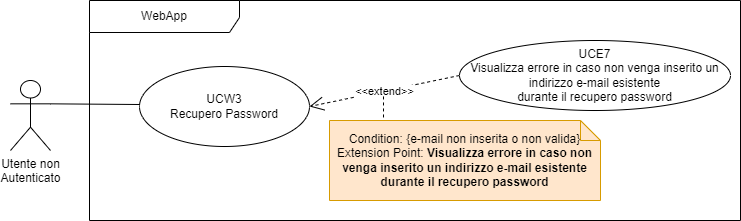
\includegraphics[scale=0.5]{UC_images/UCW3.png}
\caption{UCW3 - Recupero Password}
\end{figure}
\begin{itemize}
\item \textbf{Descrizione}: L'utente non autenticato vuole recuperare la password di accesso alla piattaforma Sweeat.
\item \textbf{Attore primario}: Utente non autenticato.
\item \textbf{Precondizione}: L’utente non è ancora autenticato presso il sistema.
\item \textbf{Postcondizione}: L’utente ha la possibilità di recuperare la password tramite l'indirizzo e-mail con cui è registrato nella piattaforma.

\item \textbf{Scenario principale}:
\begin{enumerate}
\item L’utente accede al sistema;
\item L’utente seleziona la voce “Login”;
\item L’utente clicca sulla voce “Password dimenticata”;
\item L’utente inserisce l’indirizzo e-mail da cui recuperare la password;
\item L’utente clicca su “Recupera password”. 
\end{enumerate}

\item \textbf{Estensioni}:
\begin{itemize}
\item Viene inserito un indirizzo e-mail non valido 
\begin{enumerate}
	\item L’utente non può recuperare la password;
	\item Viene mostrato un messaggio d’errore che indica che l’indirizzo e-mail inserito non è corretto (UCE7 §3.21).
\end{enumerate}
\end{itemize}
\end{itemize}

\pagebreak